\chapter{Agent Implementation Instructions}\label{ch:agent-impl}

\section{Purpose and audience}
This chapter is the self-contained, intent-based instruction set for
implementing the \emph{Trial Balance review} domain inside the
unified SAP OSS platform. It is written for LLM-driven and human
implementation agents who will extend existing services to realise
the specification. It assumes only this PDF; every platform
decision, integration contract, and governance obligation the TB
workstream depends on is restated here so that no companion document
is required. Existing chapters~\ref{ch:overview}--\ref{ch:tb-roadmap}
remain the normative source for the TB domain itself; this chapter
tells future agents \emph{how} to build what those chapters
describe, \emph{where} to put it in the codebase, and \emph{how} it
plugs into the wider platform.

% !TEX root = ../master.tex
% =============================================================================
% MASTER PLATFORM CORE: Shared Intent-Based Instructions (Union)
% World-Class Version: HITL Gates, Process Integrity, and .clinerules Wiring
% =============================================================================

\section{Rules of Engagement for AI Agents}
\label{sec:agent-rules}

To ensure safety and architectural integrity, all implementation agents must adhere to the following Prime Directives:

\begin{enumerate}[label=\textsc{rule}-\arabic*:, leftmargin=2cm]
    \item \textbf{Credential Protection.} Never log, print, or commit secrets. Use the \texttt{.secrets.example} pattern for all new integrations.
    \item \textbf{Context Efficiency.} Prioritize surgical edits. Request only the minimum required file ranges to satisfy the task intent.
    \item \textbf{Test-Driven Implementation.} No code is complete without a corresponding fixture in \texttt{tests/fixtures/} and a passing validation run.
    \item \textbf{Self-Correction.} If a schema validation fails, the agent must diagnose the root cause (hallucination vs. schema drift) before re-attempting implementation.
    \item \textbf{Safety Inheritance.} Domain-specific agent rules (\texttt{.clinerules}) may only \emph{tighten} (e.g., lower timeout, stricter precision), never \emph{loosen} regulatory constraints.
\end{enumerate}

\section{Agent Rule-Pack Architecture (.clinerules)}
\label{sec:agent-rule-packs}

The platform mandates a three-tier inheritance hierarchy for agent behavior. Implementation agents must load the relevant rule pack before starting any task.

\subsection{Inheritance Hierarchy}
\begin{enumerate}
    \item \textbf{Repository-level (\texttt{/.clinerules}):} The baseline for all engineering and documentation standards.
    \item \textbf{Intelligence-level (\texttt{/src/intelligence/.clinerules}):} The regulatory envelope (MAS MGF) that wraps all domains.
    \item \textbf{Domain-level (\texttt{/src/<domain>/.clinerules}):} Domain-specific constraints (e.g., Arabic character precision).
\end{enumerate}

\subsection{Safety-Critical Flags}
The following flags in the rule packs are subject to \textsc{rule-5} (Inherit, Never Weaken):
\begin{table}[htbp]
\centering
\footnotesize
\caption{Safety-Critical Agent Flags.}
\label{tab:safety-flags}
\begin{tabularx}{\textwidth}{@{}l X X@{}}
\toprule
\textbf{Flag} & \textbf{Parent Value (Regs)} & \textbf{Tightening Direction} \\
\midrule
\texttt{deny\_by\_default} & \texttt{true} & Invariant (Cannot be set to false). \\
\texttt{require\_identity} & \texttt{true} & Invariant (Cannot be bypassed). \\
\texttt{max\_retries} & \texttt{3} & May only \emph{decrease}. \\
\texttt{timeout\_ms} & \texttt{30000} & May only \emph{decrease}. \\
\bottomrule
\end{tabularx}
\end{table}

\section{Platform Overview --- One Codebase, One Instance}
\label{sec:agent-platform-overview}

\subsection{Integration Stance}
The SAP OSS platform is delivered as a single codebase that runs as a single logical instance. All cross-cutting concerns are hosted by existing services.

\begin{adrbox}{{One Codebase, One Instance}}
To minimize integration latency and eliminate distributed-system failure modes (e.g., partial partitions), we mandate a single logical instance. All cross-domain orchestration happens via the MCP Gateway layer.
\end{adrbox}

\subsection{Platform Integration Map}
\label{sec:platform-map}

\begin{figure}[htbp]
\centering
\begin{tikzpicture}[
    node distance=2.5cm, 
    auto,
    block/.style={rectangle, draw, rounded corners, fill=sapblue!10, text width=6em, text centered, minimum height=3em, font=\scriptsize},
    regs/.style={rectangle, draw, rounded corners, fill=sapgrey!20, text width=7em, text centered, minimum height=4em, thick, dotted, font=\scriptsize}
]
    \node (arabic) [block] {Arabic AP};
    \node (tb) [block, below of=arabic] {Trial Balance};
    \node (simula) [block, right of=arabic, node distance=5.5cm] {Simula Training};
    \node (regs) [regs, below of=simula] {Regulations (Runtime Wrapper)};
    
    \draw [->, thick] (arabic) -- node [align=left, font=\tiny] {Posted\\Invoices} (tb);
    \draw [->, thick, dashed] (simula) -- node [align=left, font=\tiny, near start] {Training\\Examples} (arabic);
    \draw [->, thick, dashed] (simula) -- node [align=left, font=\tiny, near start] {Training\\Examples} (tb);
    \draw [->, thick] (regs) -| node [font=\tiny, near end, xshift=-1cm] {Governance Gate} (arabic);
    \draw [->, thick] (regs) -| node [font=\tiny, near end, xshift=-1cm] {Audit \& Identity} (tb);
\end{tikzpicture}
\caption{Cross-domain interaction and unified data flow map. Detailed governance logic is defined in \cref{reg:ch:mgf}.}
\end{figure}

\section{Transactional Sequence Diagrams}
\label{sec:agent-sequences}

Implementation agents must adhere to the temporal logic defined below. Every cross-domain request MUST be brokered by the Regulations Wrapper.

\subsection{Universal Governance Handshake}
This sequence applies to \textbf{all} platform service calls.

\begin{figure}[htbp]
\centering
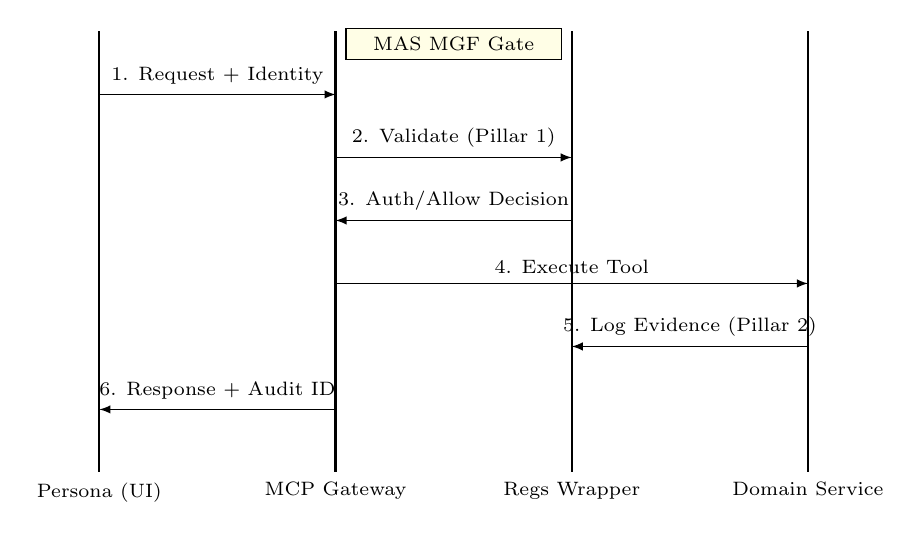
\begin{tikzpicture}[x=1cm, y=-0.8cm, font=\scriptsize]
    % Lifelines
    \draw[thick] (0,0) -- (0,7) node[below] {Persona (UI)};
    \draw[thick] (3,0) -- (3,7) node[below] {MCP Gateway};
    \draw[thick] (6,0) -- (6,7) node[below] {Regs Wrapper};
    \draw[thick] (9,0) -- (9,7) node[below] {Domain Service};

    % Interaction
    \draw[->, >=latex] (0,1) -- node[above] {1. Request + Identity} (3,1);
    \draw[->, >=latex] (3,2) -- node[above] {2. Validate (Pillar 1)} (6,2);
    \draw[<-, >=latex] (3,3) -- node[above] {3. Auth/Allow Decision} (6,3);
    \draw[->, >=latex] (3,4) -- node[above] {4. Execute Tool} (9,4);
    \draw[->, >=latex] (9,5) -- node[above] {5. Log Evidence (Pillar 2)} (6,5);
    \draw[<-, >=latex] (0,6) -- node[above] {6. Response + Audit ID} (3,6);

    \node[draw, fill=yellow!10, text width=2.5cm, align=center] at (4.5,0.2) {MAS MGF Gate};
\end{tikzpicture}
\caption{Standard platform handshake for governed tool execution. Audit schemas are detailed in \cref{reg:ch:identity}.}
\end{figure}

\subsection{Arabic AP Golden Path}
Temporal flow for invoice processing with Arabic context.

\begin{figure}[htbp]
\centering
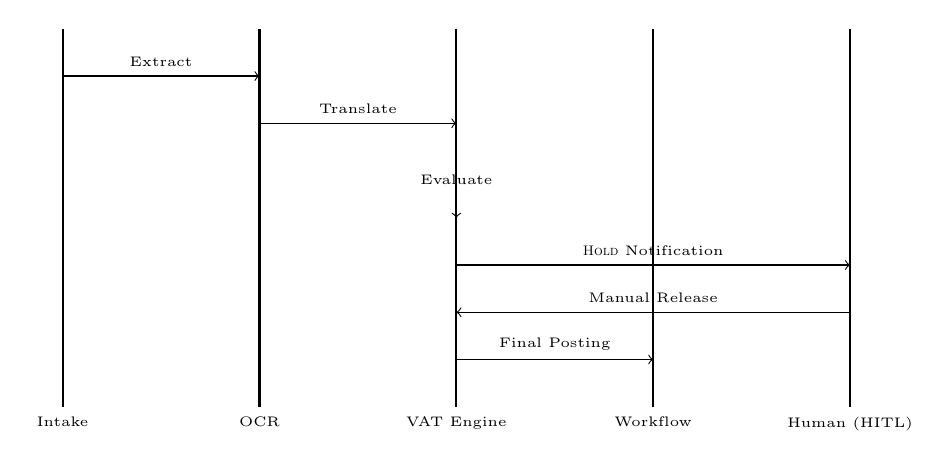
\begin{tikzpicture}[x=1cm, y=-0.6cm, font=\tiny]
    \draw[thick] (0,0) -- (0,8) node[below] {Intake};
    \draw[thick] (2.5,0) -- (2.5,8) node[below] {OCR};
    \draw[thick] (5,0) -- (5,8) node[below] {VAT Engine};
    \draw[thick] (7.5,0) -- (7.5,8) node[below] {Workflow};
    \draw[thick] (10,0) -- (10,8) node[below] {Human (HITL)};

    \draw[->] (0,1) -- node[above] {Extract} (2.5,1);
    \draw[->] (2.5,2) -- node[above] {Translate} (5,2);
    \draw[->] (5,3) -- node[above] {Evaluate} (5,4); % Internal loop
    \draw[->] (5,5) -- node[above] {\textsc{Hold} Notification} (10,5);
    \draw[<-] (5,6) -- node[above] {Manual Release} (10,6);
    \draw[->] (5,7) -- node[above] {Final Posting} (7.5,7);
\end{tikzpicture}
\caption{Arabic AP sequence: Scanned PDF to Release. VAT rules are specified in \cref{ar:ch:vat}.}
\end{figure}

\section{Compute and Resource Alignment}
\label{sec:hardware-profiles}

AI algorithms are calibrated for the reference infrastructure established in the domain chapters:

\begin{table}[htbp]
\centering
\footnotesize
\caption{Infrastructure Reference Profiles.}
\label{tab:hardware-profiles}
\begin{tabularx}{\textwidth}{@{}l X X@{}}
\toprule
\textbf{Workload} & \textbf{Reference Hardware} & \textbf{Performance Target} \\
\midrule
LLM Inference & NVIDIA L40S (48GB) & AWQ 4-bit / p95 < 2s \\
Embeddings & NVIDIA A100 (40/80GB) & FP16 / p99 < 500ms \\
Simula Training & NVIDIA A100 SXM4 cluster & BF16 throughput parity \\
\bottomrule
\end{tabularx}
\end{table}

\section{Human-in-the-Loop (HITL) Critical Gates}
\label{sec:hitl-gates}

The following "Four-Eyes" gates are mandatory. AI agents must implement the "Awaiting Sign-off" state for these actions:
\begin{itemize}
    \item \textbf{VAT Release:} No invoice marked as \textsc{hold} can be released without human review (see \cref{ar:ch:ap}).
    \item \textbf{Anomaly Override:} Statistical outliers ($3\sigma$) cannot be dismissed by AI; only "Confirmed" or "Triaged" by human (see \cref{tb:ch:controls}).
    \item \textbf{Journal Posting:} Agents may \emph{draft} journal entries, but only the Financial Controller persona can \emph{commit} to S/4HANA (see \cref{tb:ch:controls-engine}).
\end{itemize}

\section{Registry Integrity \& Live Status}
\label{sec:registry-integrity}

Before initiating any schema-dependent task, implementation agents must verify the live status of the Unified Schema Registry (see \cref{sim:chap:schema}).
\begin{adrbox}{Registry First}
If \texttt{docs/schema/registry.json} is out of sync with the codebase, the agent must halt and emit a \textsc{schema-mismatch} event.
\end{adrbox}

\section{Master Implementation Manifest (Union)}
Implementation runs in three waves across the entire platform.

\subsection*{Wave 1 --- Foundations}
\begin{itemize}
    \item \textbf{Simula:} Implement HANA schema extraction pipeline (MCP discovery). See \cref{sim:chap:extraction}.
    \item \textbf{Regulations:} Implement MAS MGF Pillar 1 logic (Tool allow-list). See \cref{reg:ch:mgf}.
    \item \textbf{Arabic:} Implement Invoice Intake \& OCR Gateway. See \cref{ar:ch:ai}.
    \item \textbf{Trial Balance:} Implement identity-attribution wiring. See \cref{reg:ch:identity}.
\end{itemize}

\subsection*{Wave 2 --- Core Domain Build-out}
\begin{itemize}
    \item \textbf{Trial Balance:} Implement Controls \& Commentary Engine (3$\sigma$ anomaly logic). See \cref{tb:ch:ai,tb:ch:controls-engine}.
    \item \textbf{Arabic:} Implement multi-country VAT Engine (Saudi, UAE, Bahrain, Oman). See \cref{ar:ch:vat,ar:ch:vat-impl}.
    \item \textbf{Simula:} Implement Taxonomy Generation \& Agentic Data Synthesis. See \cref{sim:chap:taxonomy,sim:chap:generator}.
    \item \textbf{Trial Balance:} Realise 28-state BPMN workflow (\texttt{tb-review-glo}). See \cref{tb:ch:workflow}.
\end{itemize}

\subsection*{Wave 3 --- Hardening}
\begin{itemize}
    \item \textbf{Regulations:} Implement Per-Request Identity Attribution. See \cref{reg:ch:identity}.
    \item \textbf{Trial Balance:} Deliver Human Review Dashboard. See \cref{tb:ch:review-dashboard}.
    \item \textbf{Simula:} Deliver test fixtures and testing at 85\% coverage. See \cref{sim:ch:test-fixtures,sim:ch:testing}.
    \item \textbf{Regulations:} Wire Emergent-Capability monitoring. See \cref{reg:ch:monitoring}.
\end{itemize}

\section{Governance Obligations (MAS MGF)}
The regulations domain wraps all service calls at runtime. Agents must implement the following hooks in every domain:
\begin{itemize}
    \item \textbf{Pillar 1:} Tool allow-list enforcement (deny-by-default).
    \item \textbf{Pillar 2:} Traceability via the identity attribution envelope.
    \item \textbf{Pillar 3:} Metric emission to the monitoring sink.
\end{itemize}
Detailed pillar requirements are defined in \cref{reg:ch:mgf}.


\section{FMEA: Failure Mode and Effects Analysis for AI}
\label{sec:fmea-ai}

The following analysis identifies critical AI failure modes within the TB pipeline and their deterministic mitigations.

\begin{table}[htbp]
\centering
\footnotesize
\caption{FMEA for Trial Balance AI Pipeline.}
\label{tab:tb-fmea}
\begin{tabularx}{\textwidth}{@{}l X X X@{}}
\toprule
\textbf{Failure Mode} & \textbf{Symptom} & \textbf{Impact} & \textbf{Technical Mitigation} \\
\midrule
LLM Hallucination & Commentary references accounts not in the input TB. & High (Inaccuracy) & Cross-check extracted accounts against the input TB record. \\
Normality Drift & $3\sigma$ fails due to non-normal variance distribution. & Medium (False Neg.) & Fallback to MAD (Median Absolute Deviation) scoring. \\
Prompt Injection & Malicious input triggers unverified journal posting. & Critical (Security) & Deterministic rule-check gate on all POST endpoints. \\
\bottomrule
\end{tabularx}
\end{table}

\section{This domain in context}
\label{sec:agent-domain-context}
Trial Balance review is the finance close workstream among the four
domains. Its primary persona is the Financial Controller, whose
working view is the review dashboard surfaced through the shared
workspace shell and gated by TB entitlements. The domain's entry
points are the TB extract feed and the upstream AP postings
(including those produced by the Arabic domain); its exit points are
(a)~signed-off commentary records, (b)~evidenced controls for the
month-end close, and (c)~any journal corrections posted back to SAP
S/4HANA. Every artefact is validated against the TB-owned schemas in
\texttt{structured/schema/} before it leaves the service. The domain
depends on the horizontal regulations wrapper for runtime governance
and on Simula for the training corpus used by the anomaly-detection
and commentary models described in chapter~\ref{ch:ai}.

\section{Schema contribution}
\label{sec:agent-schema-contrib}
TB owns the schemas catalogued in chapter~\ref{ch:schema} and listed
in~\ref{tab:schemas}. The canonical set is the control record
(\S\ref{sec:control-schema}, fields in~\ref{tab:control-fields}), the
decision-point record (\S\ref{sec:decision-point-schema}), the
workflow record (\S\ref{sec:workflow-schema},
header fields in~\ref{tab:workflow-fields}), and TB's own
\texttt{requirement.schema.json}. These schemas live under
\texttt{docs/latex/specs/tb/} as normative text and under
\texttt{structured/schema/} as the JSON Schema artefacts consumed at
runtime. Registration in the unified registry is additive: each
schema is listed in
\texttt{src/intelligence/ai-core-pal/data\_products/registry.yaml}
with its URI, owning domain (\texttt{tb}), security class
(\texttt{confidential}), and LLM routing (\texttt{vllm-only}),
following the ODPS~4.1 pattern. Simula consumes these schemas
directly as inputs to its extraction pipeline; it does not transform
them. TB's \texttt{requirement.schema.json} is a distinct URI from
regulations' \texttt{requirement.schema.json}; the two files are not
merged.

\section{Persona and MCP allow-list}
\label{sec:agent-persona}
\begin{itemize}
  \item \textbf{Persona id:} \texttt{financial-controller}.
  \item \textbf{Roles:} TB ingestion and validation, anomaly triage,
    commentary drafting and review, control evidencing, close
    sign-off.
  \item \textbf{Entitlements:} read/write on the TB control record,
    decision-point record, and workflow record; advance transitions
    on the 28 states of \texttt{tb-review-glo}
    (chapter~\ref{ch:workflow},~\ref{tab:states}); evidence-write on
    the control enforcement map in~\ref{fig:controls-map}; journal
    posting on corrected entries (chapter~\ref{ch:controls-engine}).
  \item \textbf{UI route:} \texttt{/tb/\{tenant\}/review} on the
    shared workspace shell; surfaced only to callers whose
    entitlement set includes \texttt{financial-controller}.
  \item \textbf{MCP tool allow-list:}
    \texttt{tb.ingest}, \texttt{tb.anomaly.detect},
    \texttt{tb.commentary.draft}, \texttt{tb.commentary.validate},
    \texttt{tb.workflow.advance}, \texttt{tb.control.evidence},
    \texttt{tb.journal.post}. All other MCP tools are denied by
    default per MAS MGF pillar~1.
\end{itemize}

\section{Agent Rule-Pack Binding}
\label{sec:agent-rule-binding}
Before initiating any task in this domain, the agent MUST load the following rule packs in order:
\begin{enumerate}
  \item \filepath{.clinerules} (Global Standards)
  \item \filepath{src/intelligence/.clinerules} (Regulations Envelope)
  \item \filepath{src/tb/.clinerules} (TB Domain Constraints)
\end{enumerate}

\section{Implementation tasks for this domain}
\label{sec:agent-tasks}
The tasks below are intent-based: each task states the outcome a
future agent must achieve and the location in the existing codebase
where the work belongs. None of them contains code; each task binds
to the TB chapters that define the required behaviour.

\subsection*{Task T1 --- Controls and commentary engine}
\textbf{Intent.} Implement the controls and commentary engine
specified in chapter~\ref{ch:controls-engine}, including the decision
tree (\ref{fig:decision-tree}), the rule format, materiality
thresholds, and journal posting.

\begin{adrbox}{Why 3-Sigma?}
We chose $3\sigma$ for v1.0 to ensure immediate baseline stability. This statistical floor provides a 99.7\% confidence interval for known variance patterns while the ML training set accumulates.
\end{adrbox}

\textbf{In-scope.} Per-rule evaluators for the anomaly checks in
~\ref{tab:anomalies} (3$\sigma$, MAD, percentile); materiality-aware
commentary generation; deadline-aware investigation routing.
\textbf{Out-of-scope.} The v2.0 ML-based anomaly detection explored
in chapter~\ref{ch:future-ml}; that work is reserved for a later
release and must remain behind a feature flag.
\textbf{Paths to extend.} AI pipeline stages in
chapter~\ref{ch:ai}, specifically stage~2 (anomaly detection) and
stage~3 (commentary drafting); engine module colocated with the
gateway service.
\textbf{Definition of done.} Every anomaly check
in~\ref{tab:anomalies} has a callable rule; commentary draft records
validate against the TB schema set and carry the evidencing required
by chapter~\ref{ch:controls-engine}.

\textbf{Autonomous Verification (Agent Logic):}
\begin{lstlisting}[language=jsonx]
// Verify Task T1
{
  "test_fixture": "tests/fixtures/tb/golden_sample.json",
  "expected_outcome": "anomaly_count == 5",
  "validation_command": "pytest src/tb/engine_test.py --verify-rules"
}
\end{lstlisting}

\textbf{Verification.} Unit tests for each rule pass; the commentary
draft endpoint produces records that pass validation.

\subsection*{Task T2 --- 28-state BPMN workflow}
\textbf{Intent.} Realise the \texttt{tb-review-glo} workflow in
chapter~\ref{ch:workflow}, including all 28 states
in~\ref{tab:states} and the preparation
(\ref{fig:prep-phase}), analysis (\ref{fig:analysis-phase}), and
sign-off phases.
\textbf{In-scope.} State transitions, phase gates, deadline handling,
roll-back and park semantics.
\textbf{Out-of-scope.} BPMN-driven cross-tenant orchestration; the
workflow runs within a single tenant per instance.
\textbf{Paths to extend.} Workflow engine hosted in the gateway
service; workflow record defined in chapter~\ref{ch:schema}.
\textbf{Definition of done.} All 28 states are reachable from a
deterministic predecessor; every transition is audit-logged with the
persona id; rolling the golden sample through the workflow produces
the signed-off close artefact without manual intervention.
\textbf{Verification.} Workflow unit tests pass; the review-dashboard
chapter (\ref{ch:review-dashboard}) queue view surfaces the expected
filter counts.

\subsection*{Task T3 --- Review dashboard}
\textbf{Intent.} Deliver the human review dashboard specified in
chapter~\ref{ch:review-dashboard}.
\textbf{In-scope.} Queue view with the fields in~\ref{tab:queue-fields},
sorting/filtering, bulk operations, review view, commentary
composition aids, sign-off flow.
\textbf{Out-of-scope.} Mobile layouts; cross-period comparative
analytics beyond what chapter~\ref{ch:review-dashboard} lists.
\textbf{Paths to extend.} Persona surface within
\texttt{generativeUI/training-webcomponents-ngx}; data-fetching
hooks that call the TB MCP tools enumerated above.
\textbf{Definition of done.} The dashboard renders the queue view,
supports the bulk operations listed in the chapter, and writes
control-evidence records through the allow-listed MCP tools.
\textbf{Verification.} Dashboard component tests pass; the persona
entitlement gate returns 403 for non-Financial-Controller callers.

\subsection*{Task T4 --- Controls and acceptance}
\textbf{Intent.} Wire the control enforcement map and acceptance
criteria in chapter~\ref{ch:controls}, including the EUC evidencing
requirement in~\ref{sec:controls-eucs}.
\textbf{In-scope.} Control-to-state binding per~\ref{fig:controls-map};
risk register mitigations from~\ref{tab:risks}; EUC evidencing hooks.
\textbf{Out-of-scope.} External SOX reporting system integration.
\textbf{Paths to extend.} Control catalogue file referenced in
chapter~\ref{ch:controls}; evidence store.
\textbf{Definition of done.} Every control fires on its bound
states; evidence records are produced; the acceptance criteria
checklist in chapter~\ref{ch:controls} is satisfied.
\textbf{Verification.} Running the TB golden sample triggers every
control; the evidence report reconciles with the acceptance
checklist.

\subsection*{Task T5 --- Testing and coverage}
\textbf{Intent.} Deliver the testing specification in
chapter~\ref{ch:testing} at the coverage thresholds
in~\ref{tab:tb-coverage}.
\textbf{In-scope.} TB extract fixtures, variance fixtures, unit
tests for variance detection and commentary drafting, integration
tests through the workflow, regression fixtures.
\textbf{Out-of-scope.} Load and performance benchmarking beyond what
chapter~\ref{ch:testing} defines.
\textbf{Paths to extend.} Test directory colocated with the TB
service code; fixture store used by Simula as training input.
\textbf{Definition of done.} Coverage meets the thresholds
in~\ref{tab:tb-coverage}; CI gates block regressions.
\textbf{Verification.} \texttt{make spec-tb} remains green; the TB
test entry points listed in chapter~\ref{ch:testing} all run.


\section{Governance obligations applied to this domain}
\label{sec:agent-governance}
The regulations domain wraps Trial Balance review at runtime. Four
obligations apply without exception; each is stated as a concrete
hook in the TB codebase.

\begin{itemize}
  \item \textbf{MAS MGF four pillars} (see regulations
    chapter~3 in
    \texttt{docs/latex/specs/regulations/chapters/03-mgf-framework.tex}).
    Pillar~1 (assess and bound): every TB MCP tool is declared in the
    allow-list in \S\ref{sec:agent-persona}, deny-by-default.
    Pillar~2 (design and deploy): the pipeline stages in
    chapter~\ref{ch:ai} are traceable end-to-end via the per-request
    identity attribution described below. Pillar~3 (operate and
    monitor) and pillar~4 (govern and disclose) are satisfied by
    emitting the evidence records produced by the TB control
    catalogue (chapter~\ref{ch:controls}) into the shared governance
    store.
  \item \textbf{Identity attribution} (regulations chapter~10,
    \texttt{10-identity-attribution.tex}). Every MCP call and every
    workflow transition carries the persona id, agent id, request id,
    and tenant id. The gateway is the attachment point; TB code
    propagates the identity envelope without mutating it.
  \item \textbf{Emergent-capability monitoring} (regulations
    chapter~8, \texttt{08-monitoring-spec.tex}). Anomaly detection,
    commentary drafting, and workflow state transitions are
    instrumented with the monitoring metrics specified in that
    chapter; metrics flow to the monitoring sink defined there.
  \item \textbf{Conformance tooling} (regulations chapter~6,
    \texttt{06-conformance-tooling.tex}). The TB service exposes
    AI Verify 2.0 plug-in hooks and Moonshot CI/CD 1.1.0 benchmark
    entry points as required by that chapter.
\end{itemize}

\section{Cross-spec integration --- full detail}
\label{sec:agent-integration}

\subsection{With Arabic AP}
Arabic AP produces posted AP records and VAT checklists that feed
the TB close. TB consumes them as evidence inputs to its commentary
engine, not as schema merges: the Arabic invoice schema and the TB
control record remain distinct URIs in the unified registry.
Integration point: TB's ingestion stage calls the Arabic MCP tool
\texttt{invoice.extract-fields} with read-only entitlements; the
response is validated against \texttt{invoice.schema.json} before TB
accepts it.

\subsection{With Trial Balance}
TB exports the control record, decision-point record, workflow
record, and its own \texttt{requirement.schema.json} under
\texttt{structured/schema/} (chapter~\ref{ch:schema}); registers the
MCP tools enumerated in \S\ref{sec:agent-persona}; and applies the
four governance hooks in \S\ref{sec:agent-governance} to every call
it serves. External consumers (Arabic, regulations, Simula) see TB
only through these contracts; there are no private back-channels.

\subsection{With Regulations}
Regulations wraps TB at runtime. Every TB MCP call is brokered
through the regulations governance gate, which applies pillars~1--4
of MAS MGF, attaches the identity envelope, and routes
emergent-capability metrics to the monitoring store. The TB service
code does not call regulations directly; the gateway layer enforces
this. Conformance tests defined in regulations chapter~5 (empirical
evidence) and chapter~6 (conformance tooling) execute against the TB
service as part of the platform CI gate.

\subsection{With Simula}
Simula consumes TB's schemas and fixtures as training input. The
contract is schema-in, \texttt{TrainingExample}-out: Simula reads the
TB schema set and the TB fixture store; it produces
\texttt{TrainingExample} records. Simula does not call TB MCP tools
at runtime and does not share state with the TB workflow. No
cross-domain operational envelope is introduced.

\section{Wave assignment and sequencing}
\label{sec:agent-waves}
Implementation runs in three waves.

\begin{itemize}
  \item \textbf{Wave 1 --- foundations.} Unified schema registry
    entry; persona-gated surface for the Financial Controller;
    identity attribution envelope flowing through the gateway.
    Prerequisites: the regulations chapter~10 identity schema must
    be frozen.
  \item \textbf{Wave 2 --- TB core build-out.} Tasks T1, T2, T3, T4
    above. Prerequisites: Wave~1 complete; Simula training fixtures
    available from Simula Wave~1 (extraction pipeline); Arabic MCP
    tool \texttt{invoice.extract-fields} reachable.
  \item \textbf{Wave 3 --- hardening and conformance.} Task T5 and
    full conformance-tooling hook-up. Prerequisites: Wave~2 complete;
    regulations Wave~2 conformance tooling integrated; monitoring
    sink live.
\end{itemize}

TB occupies Wave~2 for its core build-out and Wave~3 for its testing
and conformance surfaces.

\section{Acceptance criteria (platform-wide)}
\label{sec:agent-acceptance}
When all four chapter~12 instruction sets are implemented, the
platform satisfies the following invariants:

\begin{enumerate}
  \item \textbf{One instance.} A single codebase runs a single
    logical instance; no domain ships as a separate product.
  \item \textbf{Persona-gated surfaces.} The four personas each
    reach a tailored UI on the shared shell; no route, MCP tool, or
    data product is visible outside its persona's entitlement set.
  \item \textbf{Unified registry.} Every schema in use is listed in
    the ODPS~4.1 registry under its owning domain; validators
    resolve \texttt{\$ref}s through the unified registry only.
  \item \textbf{No schema merges.} The two
    \texttt{requirement.schema.json} files in TB and regulations
    remain distinct; no cross-domain composite schemas are produced.
  \item \textbf{No cross-domain operational envelope.} Runtime
    orchestration stays within each domain's service; only Simula
    consumes other domains' outputs, and only as training input.
  \item \textbf{Governance wraps all three non-regulations domains.}
    Arabic, TB, and Simula service calls pass through the
    regulations runtime wrapper without exception.
  \end{enumerate}

\section{References}
\label{sec:agent-references}
Within-spec references:
chapter~\ref{ch:overview} (overview),
chapter~\ref{ch:schema} (data schema),
chapter~\ref{ch:ai} (AI augmentation pipeline),
chapter~\ref{ch:controls-engine} (controls and commentary engine),
chapter~\ref{ch:workflow} (workflow and approval engine),
chapter~\ref{ch:controls} (controls, testing and acceptance),
chapter~\ref{ch:references} (references),
chapter~\ref{ch:review-dashboard} (review dashboard),
chapter~\ref{ch:testing} (testing specification),
chapter~\ref{ch:future-ml} (future ML work),
chapter~\ref{ch:tb-roadmap} (project roadmap).

Peer chapter~12 instruction sets for the other three domains (each
is self-contained; consult directly when operating in that domain):
\begin{itemize}
  \item Arabic AP:
    \texttt{docs/latex/specs/arabic/chapters/12-implementation-instructions.tex}.
  \item Regulations:
    \texttt{docs/latex/specs/regulations/chapters/12-implementation-instructions.tex}.
  \item Simula:
    \texttt{docs/latex/specs/simula/chapters/12-implementation-instructions.tex}.
\end{itemize}

Shared platform artefacts:
\begin{itemize}
  \item ODPS~4.1 registry:
    \texttt{src/intelligence/ai-core-pal/data\_products/registry.yaml}.
  \item Schema pipeline and resolver:
    \texttt{src/intelligence/schema\_pipeline/}.
  \item Training pipeline (Simula):
    \texttt{src/training/pipeline/}.
  \item Shared workspace shell:
    \texttt{generativeUI/training-webcomponents-ngx}.
\end{itemize}
